\documentclass[conference]{IEEEtran}
% Compile: tectonic main.tex   (or pdflatex + bibtex on Overleaf)
% All numbers in tables and in the text come from build_paper_assets.py (tables/*.tex, numbers.tex).

\usepackage{cite}
\usepackage{amsmath,amssymb}
\usepackage{newtxtext,newtxmath} % Times text and math, as in IEEE publications
\usepackage{graphicx}
\usepackage{booktabs}
\usepackage{xcolor}
\usepackage{url}
\usepackage{tikz}
\usetikzlibrary{positioning,arrows.meta}
\usepackage[hidelinks]{hyperref}
% Auto-generated by build_paper_assets.py -- do not edit by hand.
\newcommand{\nCleanMIoU}{79.35}
\newcommand{\nCleanLo}{77.34}
\newcommand{\nCleanHi}{81.01}
\newcommand{\nCleanMDice}{88.27}
\newcommand{\nCleanAnat}{87.84}
\newcommand{\nCleanInst}{75.71}
\newcommand{\nPGDOne}{4.35}
\newcommand{\nPGDOneFall}{94.5}
\newcommand{\nSegOne}{3.88}
\newcommand{\nSegOneFall}{95.1}
\newcommand{\nPGDEight}{0.39}
\newcommand{\nPGDEightFall}{99.5}
\newcommand{\nSegEight}{0.34}
\newcommand{\nSegEightFall}{99.6}
\newcommand{\nFGSMOne}{56.28}
\newcommand{\nFGSMOneFall}{29.1}
\newcommand{\nFGSMEight}{55.06}
\newcommand{\nFGSMEightFall}{30.6}
\newcommand{\nNoiseOne}{79.17}
\newcommand{\nNoiseOneFall}{0.2}
\newcommand{\nNoiseEight}{75.20}
\newcommand{\nNoiseEightFall}{5.2}
\newcommand{\nFGSMFallMin}{29.1}
\newcommand{\nFGSMFallMax}{30.6}
\newcommand{\nIterFallMin}{94.5}
\newcommand{\nIterFallMax}{99.6}
\newcommand{\nPSNRPGDOne}{51.2}
\newcommand{\nPSNRFGSMOne}{48.2}
\newcommand{\nCWSegMin}{68}
\newcommand{\nCWSegMax}{77}
\newcommand{\nCWPGDMin}{63}
\newcommand{\nCWPGDMax}{71}
\newcommand{\nPGDQ}{21.23}
\newcommand{\nPGDQFall}{73.2}
\newcommand{\nSegQ}{21.36}
\newcommand{\nSegQFall}{73.1}
\newcommand{\nFGSMQ}{62.81}
\newcommand{\nFGSMQFall}{20.8}
\newcommand{\nQuantMax}{0.26}
\newcommand{\nGapNoiseEight}{3.6}
\newcommand{\nGapFGSMQ}{8.2}
\newcommand{\nGapFGSMEight}{16.7}
\newcommand{\nGapFGSMOne}{11.8}
\newcommand{\nGapPGDQ}{20.7}
\newcommand{\nGapSegQ}{16.1}
\newcommand{\nGapPGDOne}{8.4}
\newcommand{\nGapSegOne}{5.8}
\newcommand{\nGapPresPGDQ}{14.6}
\newcommand{\nGapPresSegQ}{12.5}
\newcommand{\nAnatFallPGDQ}{59.4}
\newcommand{\nInstFallPGDQ}{80.1}
\newcommand{\nAnatFallFGSMOne}{21.2}
\newcommand{\nInstFallFGSMOne}{33.0}
\newcommand{\nPupilGT}{6.7}
\newcommand{\nPupilSeg}{49.5}
\newcommand{\nPupilPGD}{43.7}
\newcommand{\nInjGT}{0.1}
\newcommand{\nInjSeg}{6.0}
\newcommand{\nBgGT}{84.8}
\newcommand{\nBgSeg}{33.6}
\newcommand{\nPGDFiveOne}{22.01}
\newcommand{\nPGDFortyOne}{2.24}
\newcommand{\nPGDFiveOneFall}{72}
\newcommand{\nRhoMin}{-0.56}
\newcommand{\nRhoMax}{-0.14}
\newcommand{\nRhoPMin}{0.09}
\newcommand{\nBestEpoch}{36}
\newcommand{\nValBest}{75.82}
\newcommand{\nTrainMin}{55}
\newcommand{\nRepPGDOne}{95.0}
\newcommand{\nRepNoiseEight}{10.3}
\newcommand{\nRefIris}{79.97}
\newcommand{\nOurIris}{84.55}
\newcommand{\nRefPupil}{86.24}
\newcommand{\nOurPupil}{92.42}
\newcommand{\nRefLens}{77.23}
\newcommand{\nOurLens}{86.55}


\newcommand{\eps}{\varepsilon}
\newcommand{\pp}{\,pp}
\renewcommand{\arraystretch}{1.08}

\begin{document}

\title{Adversarial Attack and Robustness Analysis of AI-Based Cataract Surgical Instrument Segmentation}

% NOTE: confirm the author list, order and e-mail addresses before submission.
\author{
\IEEEauthorblockN{Parikshat Singh, Venu Kulshreshtha, Sayyad Ahsan, and Jolly Parikh}
\IEEEauthorblockA{Department of Computer Science and Engineering\\
Bharati Vidyapeeth's College of Engineering (affiliated to GGSIPU), New Delhi, India}
}

\maketitle

\begin{abstract}
Segmentation networks that label surgical instruments and ocular anatomy in cataract surgery videos are increasingly used as part of computer-assisted surgery systems. Existing results on the Cataract-1K dataset are, however, reported for clean frames only, and the behaviour of these models under adversarial perturbation has not been studied. In this work we train a DeepLabV3+ network with a ResNet-50 encoder on the Cataract-1K segmentation subset and evaluate it on the official held-out patient fold (561 frames), where it obtains a mean intersection-over-union (mIoU) of \nCleanMIoU\%, which is comparable to or better than the published baseline for all three anatomical structures. The model is then attacked with white-box FGSM, PGD and SegPGD perturbations with an $L_\infty$ budget of $\eps\in\{1,2,4,8\}/255$. We also include a random-noise control, a step-count ablation, budgets smaller than one 8-bit intensity level and a test with 8-bit quantised adversarial frames, which gives 41 evaluation runs in total. Changing each pixel by at most one intensity level (PSNR of about \nPSNRPGDOne\,dB) lowers the mIoU to \nPGDOne\% with PGD-20 and to \nSegOne\% with SegPGD-20, a relative drop of about 95\%, whereas random noise with eight times this budget reduces it by only \nNoiseEightFall\%. Rounding the adversarial frames to 8-bit values does not weaken the attack. Under the iterative attacks the network predicts large spurious regions and labels roughly half of all pixels as pupil. When the two groups of classes are compared within the same frames, the instruments lose a larger fraction of their clean accuracy than the cornea, pupil and lens for every type of attack, by up to \nGapPGDQ\ percentage points, and this holds in each of the six test videos even after hallucinated pixels are discounted. The main observations are also reproduced in an earlier, independent run on 908 frames. Our results show that a high clean accuracy says little about how reliable a cataract segmentation model is.
\end{abstract}

\begin{IEEEkeywords}
Adversarial robustness, semantic segmentation, cataract surgery, surgical instrument segmentation, medical image analysis, SegPGD.
\end{IEEEkeywords}

% ==============================================================================================
\section{Introduction}

Cataract surgery is one of the most common surgical procedures performed worldwide, and the video recorded through the operating microscope is now widely used for computer-assisted analysis. Many of these applications, for example instrument tracking, recognition of the surgical phase and assessment of surgical skill, depend on a pixel-level description of the scene in which each pixel is assigned to the cornea, the pupil, the intraocular lens or one of the instruments in use~\cite{ghamsarian2024cataract,sinha2025identifying}. The release of large annotated datasets such as Cataract-1K~\cite{ghamsarian2024cataract} has made it possible to train such segmentation models, and recent methods such as RP-SAM2~\cite{zhaksylyk2025rpsam2} report steady improvements in clean accuracy.

On the other hand, it is well known that deep networks can be misled by adversarial examples, that is, by inputs to which a small and carefully computed perturbation has been added~\cite{szegedy2014intriguing,goodfellow2015explaining,madry2018towards}. Such a perturbation is usually invisible to a human observer but can change the prediction completely. Semantic segmentation models are affected in the same way~\cite{xie2017adversarial,arnab2018robustness,gu2022segpgd}, and several studies have reported that models for medical images are at least as sensitive as models trained on natural images~\cite{finlayson2018adversarial,ma2021understanding,bortsova2021adversarial}. A further difficulty is that a weak attack can make a model look considerably more robust than it actually is~\cite{athalye2018obfuscated,croce2023reliable}.

To the best of our knowledge, the adversarial robustness of cataract surgical segmentation has not been evaluated so far. Work on adversarial attacks against medical segmentation has mostly used radiological volumes and diagnostic images~\cite{malik2024evaluating,dietrich2026thyroid,dong2023survey}. The main robustness benchmark for surgical tool segmentation considers only natural corruptions~\cite{ding2024segstrongc}, and adversarial studies in surgery have dealt with action recognition, tool detection and robot control on laparoscopic or robotic data~\cite{cheng2022why,khan2024guardian,jin2026telesurgery}. The models published for Cataract-1K have all been evaluated on unperturbed frames~\cite{ghamsarian2024cataract,zhaksylyk2025rpsam2}.

In this paper we measure this robustness directly, using a controlled protocol with statistical confidence estimates. The main contributions are as follows.
\begin{itemize}
\item We evaluate a strong Cataract-1K segmentation baseline under FGSM, PGD and SegPGD at four specified and two sub-8-bit budgets, together with a random-noise control, a step-count ablation and an 8-bit storage check, in 41 runs on the complete held-out fold.
\item We compare the vulnerability of the anatomical structures and of the instruments within the same frames, using paired bootstrap confidence intervals, per-video consistency and an additional analysis that separates actual segmentation errors from hallucinated predictions.
\item We analyse the type of failure and show that iterative attacks lead the model to predict large and confident but non-existent structures rather than empty masks.
\item We repeat the study on an independent 908-frame run in order to identify which of the conclusions are stable.
\end{itemize}

% ==============================================================================================
\section{Related Work}

\subsection{Cataract surgical scene segmentation}
The CATARACTS challenge~\cite{luengo2021cataracts} was one of the first efforts on semantic segmentation of cataract surgery. Cataract-1K~\cite{ghamsarian2024cataract} contains 2,256 annotated frames from 30 videos, with three anatomical and nine instrument classes and a split into five patient-disjoint folds; its authors also benchmarked eleven networks, among them DeepLabV3+. On the same data, RP-SAM2~\cite{zhaksylyk2025rpsam2} improves the stability of prompt-based segmentation with SAM2, and Sinha \emph{et al.}~\cite{sinha2025identifying} proposed a network for real-time instrument identification in cataract videos. These works focus on accuracy and stability for clean frames, and none of them reports results on perturbed inputs.

\subsection{Adversarial attacks on semantic segmentation}
The fast gradient sign method (FGSM)~\cite{goodfellow2015explaining} and projected gradient descent (PGD)~\cite{madry2018towards} are still the standard first-order attacks, while Carlini and Wagner~\cite{carlini2017towards} proposed stronger optimisation-based variants. Xie \emph{et al.}~\cite{xie2017adversarial} were the first to attack dense prediction models, and Arnab \emph{et al.}~\cite{arnab2018robustness} carried out a systematic study of the robustness of segmentation networks. SegPGD~\cite{gu2022segpgd} modifies the PGD loss by weighting correctly and incorrectly classified pixels differently, which makes the attack more effective for segmentation. Croce \emph{et al.}~\cite{croce2023reliable} showed that commonly used attacks overestimate the robustness of segmentation models. For prompt-based foundation models the situation is less clear, since FGSM and PGD are often reported to be ineffective against SAM~\cite{liu2024region}. With such a model, a small drop in accuracy could be caused by a weak attack rather than by a robust model.

\subsection{Adversarial robustness in medical imaging}
Finlayson \emph{et al.}~\cite{finlayson2018adversarial} were among the first to point out the risk of adversarial attacks for medical deep learning. Ma \emph{et al.}~\cite{ma2021understanding} reported that medical models are more vulnerable than models for natural images, and Bortsova \emph{et al.}~\cite{bortsova2021adversarial} investigated which factors influence this vulnerability. Malik \emph{et al.}~\cite{malik2024evaluating} evaluated volumetric medical segmentation under pixel-domain and frequency-domain attacks, Dietrich and McShannon~\cite{dietrich2026thyroid} examined thyroid nodule segmentation in ultrasound, and Dong \emph{et al.}~\cite{dong2023survey} give a survey of the area. All of these studies deal with diagnostic images rather than with video recorded during surgery.

\subsection{Robustness in surgical AI}
SegSTRONG-C~\cite{ding2024segstrongc} evaluates surgical tool segmentation under smoke, bleeding and low brightness, and Shen \emph{et al.}~\cite{shen2024sam2} tested SAM2 on surgical video with similar non-adversarial corruptions. Adversarial perturbations have been used to analyse surgical action-triplet recognition~\cite{cheng2022why}, a defence for tool detection in robot-assisted surgery has been proposed~\cite{khan2024guardian}, and learned telesurgery policies have been shown to be vulnerable to attacks~\cite{jin2026telesurgery}. As far as we are aware, the adversarial vulnerability of cataract scene segmentation has not been addressed, and the same holds for the question of whether anatomy and instruments in the same frame differ in their vulnerability.

% ==============================================================================================
\section{Materials and Methods}

\subsection{Dataset and split}
We used the segmentation subset of Cataract-1K~\cite{ghamsarian2024cataract}, which consists of 2,256 frames with a resolution of $1024\times768$, taken from 30 surgery videos at intervals of five seconds and annotated with Supervisely polygons. The polygons were rasterised into 13 classes, namely background, cornea (referred to as iris in~\cite{ghamsarian2024cataract}), pupil, intraocular lens (IOL) and nine instrument classes. As in the original benchmark, the slit knife and the incision knife share one class. Instruments were drawn after the anatomy, so that an instrument covering the eye keeps its own label. We followed the official protocol and used fold~1 (6 videos, 561 frames) as the held-out test set. From each of the other four folds one video was taken for validation (283 frames in total), and the remaining 20 videos were used for training (1,412 frames), so that no patient appears in more than one split. All frames were resized to $512\times512$. Two classes occur only rarely in the test fold, the slit/incision knife (12 frames) and the Katena forceps (8 frames). They are reported separately, and the headline means are computed over the other 10 foreground classes (3 anatomical and 7 instrument classes).

\subsection{Segmentation model and training}
We used DeepLabV3+~\cite{chen2018encoder} with a ResNet-50 encoder~\cite{he2016deep} pretrained on ImageNet~\cite{deng2009imagenet}, an output stride of 16, an ASPP module with rates 6, 12 and 18 and a low-level decoder, which gives 40.35\,M parameters. The ImageNet normalisation is implemented inside the model, so the network takes images in $[0,1]$ RGB space as input, and the perturbation is therefore also defined in this space. We chose DeepLabV3+ for two reasons. It is one of the architectures benchmarked in~\cite{ghamsarian2024cataract}, which allows us to compare our clean results with published numbers, and as a conventional encoder--decoder it does not share the problem of prompt-based models, for which standard attacks may be ineffective~\cite{liu2024region}.

The training loss was the sum of the cross-entropy and 0.8 times the soft Dice loss, following~\cite{ghamsarian2024cataract}. We used AdamW~\cite{loshchilov2019decoupled} with a learning rate of $10^{-4}$ for the encoder and $5\times10^{-4}$ for the decoder, a weight decay of $10^{-4}$, one epoch of linear warm-up followed by cosine decay, a batch size of 8 and 40 epochs. For augmentation we applied random flips, random affine transformations (scale 0.75--1.25, rotation $\pm15^\circ$, translation $\pm10\%$), colour jitter and, occasionally, Gaussian blur. The checkpoint with the highest validation mIoU (epoch~\nBestEpoch, \nValBest\%) was used in all experiments. Training took about \nTrainMin\,min on an NVIDIA RTX~3060 Laptop GPU.

\subsection{Threat model}
We assume a white-box attacker, who has full access to the architecture, the weights and the gradients, and whose goal is untargeted, which means that any incorrect prediction counts as a success. For a clean frame $x\in[0,1]^{3\times H\times W}$ with ground-truth mask $y$, the attacker searches for a perturbation $\delta$ with $\|\delta\|_\infty\le\eps$ and $x+\delta\in[0,1]^{3\times H\times W}$ that maximises the segmentation error. We give the budgets in 8-bit units, so that $\eps=1/255$ allows each pixel channel to change by at most one intensity level. The perturbation is added digitally to the decoded frame, before normalisation. Fig.~\ref{fig:pipeline} shows the resulting attack and evaluation loop.

\begin{figure}[t]
\centering
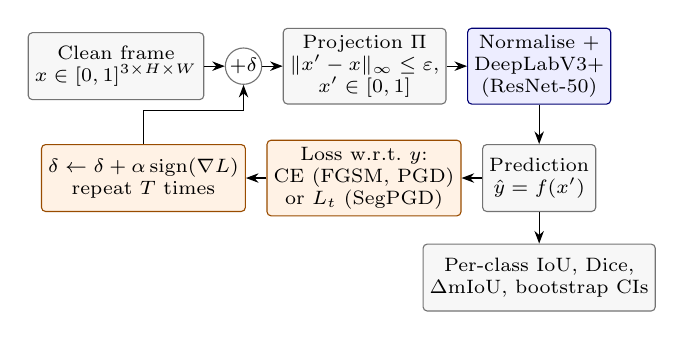
\begin{tikzpicture}[font=\scriptsize, >={Stealth[length=1.6mm]},
  box/.style={draw=black!55, rounded corners=1.5pt, align=center, inner sep=2.4pt, minimum height=8.5mm, fill=black!3},
  net/.style={box, fill=blue!7, draw=blue!45!black},
  atk/.style={box, fill=orange!10, draw=orange!60!black}]
\node[box] (x) {Clean frame\\$x\in[0,1]^{3\times H\times W}$};
\node[draw=black!55, circle, inner sep=0.6pt, right=2.6mm of x] (add) {$+\delta$};
\node[box, right=2.6mm of add] (proj) {Projection $\Pi$\\$\|x'-x\|_\infty\le\varepsilon$,\\ $x'\in[0,1]$};
\node[net, right=2.6mm of proj] (model) {Normalise +\\DeepLabV3+\\(ResNet-50)};
\node[box, below=5mm of model] (pred) {Prediction\\$\hat{y}=f(x')$};
\node[atk, left=2.6mm of pred] (loss) {Loss w.r.t.\ $y$:\\CE (FGSM, PGD)\\or $L_t$ (SegPGD)};
\node[atk, left=2.6mm of loss] (step) {$\delta\leftarrow\delta+\alpha\,\mathrm{sign}(\nabla L)$\\repeat $T$ times};
\node[box, below=4mm of pred] (eval) {Per-class IoU, Dice,\\$\Delta$mIoU, bootstrap CIs};
\draw[->] (x) -- (add);
\draw[->] (add) -- (proj);
\draw[->] (proj) -- (model);
\draw[->] (model) -- (pred);
\draw[->] (pred) -- (loss);
\draw[->] (loss) -- (step);
\draw[->] (step.north) |- ([yshift=-3.2mm]add.south) -- (add.south);
\draw[->] (pred) -- (eval);
\end{tikzpicture}
\caption{White-box attack and evaluation loop. The perturbation is added in $[0,1]$ RGB space before normalisation and is projected back onto the $L_\infty$ ball after each step. FGSM corresponds to a single step of size $\eps$.}
\label{fig:pipeline}
\end{figure}

\subsection{Attacks}
Let $L(x)=\sum_i \mathrm{CE}(f(x)_i,y_i)$ denote the pixel-wise cross-entropy summed over all pixels $i$. We use the sum instead of the mean because the sign of the gradient stays the same while numerical underflow is avoided. $\Pi$ denotes the projection onto the feasible set. \textbf{FGSM}~\cite{goodfellow2015explaining} performs a single step,
\begin{equation}
x' = \Pi\big(x + \eps\,\mathrm{sign}(\nabla_x L(x))\big).
\end{equation}
\textbf{PGD-$T$}~\cite{madry2018towards} is initialised at $x^0=\Pi(x+u)$ with $u\sim\mathcal{U}(-\eps,\eps)$ and then iterates
\begin{equation}
x^{t+1} = \Pi\big(x^t + \alpha\,\mathrm{sign}(\nabla_x L(x^t))\big),\qquad \alpha=\eps/4 .
\end{equation}
\textbf{SegPGD-$T$}~\cite{gu2022segpgd} uses the same update but changes the loss over the iterations,
\begin{equation}
L_t(x) = (1-\lambda_t)\!\!\sum_{i\in\mathcal{C}_t}\!\mathrm{CE}_i + \lambda_t\!\!\sum_{i\notin\mathcal{C}_t}\!\mathrm{CE}_i,\quad \lambda_t=\frac{t-1}{2T},
\end{equation}
where $\mathcal{C}_t$ is the set of pixels that are still classified correctly at step~$t$. In the first steps the attack therefore concentrates on pixels that have not been flipped yet. Unless stated otherwise, we use $T=20$ for both iterative attacks. As a \textbf{random-noise control} we add $\eps\,s$, where $s$ is drawn uniformly from $\{-1,+1\}$ for every pixel and channel. This perturbation has the same $L_\infty$ budget and the largest possible $L_2$ norm, but it carries no gradient information. All attacks and evaluations were run in 32-bit floating point with the model in evaluation mode. The budget and the pixel range were checked for every batch, and in every attacked run the measured $\|\delta\|_\infty$ was exactly $\eps$.

\subsection{Evaluation protocol}
Per-class IoU and Dice were computed from pixel counts accumulated over all test frames. The headline mIoU is the mean over the 10 non-rare classes, and the anatomy and instrument means are taken over the 3 and 7 classes of the respective group. As the attack does not change the ground truth, the clean and the attacked runs are averaged over exactly the same classes. We report the degradation both as $\Delta\mathrm{mIoU}=\mathrm{mIoU}_{\text{clean}}-\mathrm{mIoU}_{\text{adv}}$ and as the relative fall $\Delta\mathrm{mIoU}/\mathrm{mIoU}_{\text{clean}}$. In addition we give the fraction of pixels that were correct on the clean frame but became wrong after the attack (\emph{correct$\to$wrong}), as well as the PSNR of the adversarial frame. The 95\% confidence intervals (CIs) were obtained with a paired bootstrap over frames with 2,000 resamples~\cite{efron1993bootstrap}, in which the same resampled frames are used for the clean and for the attacked run. Since frames from the same video are correlated, we also count in how many of the six test videos an effect points in the same direction, and we report a one-sided sign test over frames. To distinguish real segmentation errors from hallucinated pixels, we further compute a \emph{present-frames-only} variant in which each class is scored only on the frames that contain it. Finally, the relation between object size and vulnerability is measured by the Spearman correlation, across classes, between the mean ground-truth area and the relative fall.

\subsection{Experiment grid}
In total we carried out 41 runs, each on all 561 test frames: the clean model; the specified grid with FGSM, PGD-20 and SegPGD-20 at $\eps\in\{1,2,4,8\}/255$; the noise control at the same budgets; step-count ablations with $T\in\{5,10,40\}$ for PGD and SegPGD at $\eps=4/255$ and $1/255$; the three attacks at the sub-8-bit budgets $\eps\in\{\frac14,\frac12\}/255$; and the three attacks at $\eps\in\{1,2\}/255$ with the adversarial frame rounded to 8-bit values before inference.

% ==============================================================================================
\section{Results}

\subsection{Clean baseline}
The clean results are listed in Table~\ref{tab:clean}. On the test fold the model reaches a headline mIoU of \nCleanMIoU\% (95\% CI \nCleanLo--\nCleanHi) and a mean Dice of \nCleanMDice\%; the mIoU is \nCleanAnat\% for the anatomical classes and \nCleanInst\% for the instruments. For all three anatomical structures the IoU is equal to or higher than the DeepLabV3+ result reported in~\cite{ghamsarian2024cataract} (iris \nOurIris\ vs.\ \nRefIris, pupil \nOurPupil\ vs.\ \nRefPupil, lens \nOurLens\ vs.\ \nRefLens). This comparison should be taken as indicative only, because~\cite{ghamsarian2024cataract} reports an average over five folds obtained with a different training procedure, whereas we evaluate on the official fold~1. The rare Katena forceps is mostly missed even on clean frames. Overall the baseline is well trained, and the vulnerability described below cannot be explained by a weak model.

\begin{table}[t]
\centering
\caption{Clean results on the held-out test fold (561 frames). IoU and Dice in \%; Frames is the number of test frames that contain the class. Ref.: DeepLabV3+ result reported in~\cite{ghamsarian2024cataract} (mean over five folds). $^\ast$Rare class, not included in the means.}
\label{tab:clean}
\footnotesize
\setlength{\tabcolsep}{4pt}
\begin{tabular}{@{}llrrrr@{}}
\toprule
Class & Group & Frames & IoU & Dice & Ref.~\cite{ghamsarian2024cataract} \\
\midrule
Cornea & Anat. & 561 & 84.55 & 91.63 & 79.97 \\
Pupil & Anat. & 561 & 92.42 & 96.06 & 86.24 \\
Lens (IOL) & Anat. & 107 & 86.55 & 92.79 & 77.23 \\
Slit/incision knife$^\ast$ & Instr. & 12 & 79.16 & 88.37 & -- \\
Gauge & Instr. & 103 & 70.37 & 82.61 & -- \\
Caps. Cystotome & Instr. & 20 & 64.64 & 78.53 & -- \\
Caps. Forceps & Instr. & 33 & 74.96 & 85.69 & -- \\
Katena Forceps$^\ast$ & Instr. & 8 & 4.08 & 7.85 & -- \\
Spatula & Instr. & 212 & 74.36 & 85.30 & -- \\
Phaco. Tip & Instr. & 148 & 82.93 & 90.67 & -- \\
Irrigation-aspiration & Instr. & 120 & 84.12 & 91.37 & -- \\
Lens Injector & Instr. & 14 & 78.61 & 88.03 & -- \\
\midrule
Instruments merged & -- & 462 & 79.34 & 88.48 & 53.53 \\
\midrule
\textbf{Headline mean} & 10 cl. & 561 & \textbf{79.35} & \textbf{88.27} & -- \\
Anatomy mean & 3 cl. & 561 & 87.84 & 93.49 & -- \\
Instrument mean & 7 cl. & 561 & 75.71 & 86.03 & -- \\
\bottomrule
\end{tabular}

\end{table}

\subsection{Vulnerability to adversarial perturbation}
Table~\ref{tab:main} and Fig.~\ref{fig:eps} give the results of the main grid. The three types of perturbation behave very differently. Random noise has almost no effect and reduces the mIoU by \nNoiseOneFall\% at $\eps=1/255$ and by \nNoiseEightFall\% at $8/255$. FGSM removes between \nFGSMFallMin\ and \nFGSMFallMax\% at every budget, and its effect does not grow with $\eps$. This is what one would expect from a single linear step, which stops being effective once the loss surface is no longer approximately linear. The iterative attacks, in contrast, make the model fail almost completely. At $\eps=1/255$, PGD-20 and SegPGD-20 lower the mIoU to \nPGDOne\% and \nSegOne\%, and at $8/255$ to \nPGDEight\% and \nSegEight\%, which corresponds to a relative fall of \nIterFallMin--\nIterFallMax\% over the specified budgets.

The comparison between noise and FGSM at $\eps=1/255$ is worth a closer look. In both cases every pixel channel is changed by exactly $\pm1/255$ (PSNR \nPSNRFGSMOne\,dB), but the noise costs only \nNoiseOneFall\% of the mIoU while FGSM costs \nFGSMOneFall\%. The model is therefore sensitive to the direction of the perturbation and not to small perturbations in general. The PGD perturbations are even harder to see (\nPSNRPGDOne\,dB at $1/255$, since not all pixels reach $\pm\eps$), and yet they do roughly three times as much damage as FGSM. Because the iterative attacks were already saturated at the smallest specified budget, we added two smaller budgets. Even at $\eps=\frac14/255$, PGD-20 still removes \nPGDQFall\% of the mIoU (Fig.~\ref{fig:eps}).

\begin{table*}[t]
\centering
\caption{Results on the held-out test fold (561 frames) without and with attack. PGD and SegPGD use $T=20$, $\alpha=\eps/4$ and a random start. The CIs were obtained with a paired bootstrap over frames (2,000 resamples). Corr.$\to$wrong: fraction of pixels that were correct on the clean frame and are wrong after the attack.}
\label{tab:main}
\footnotesize
\setlength{\tabcolsep}{5pt}
\begin{tabular}{@{}llrrrrrrrr@{}}
\toprule
Attack & $\varepsilon$ & mIoU [95\% CI] & $\Delta$mIoU & Rel. fall & mDice & Anat. & Instr. & Corr.$\to$wrong & PSNR \\
 & ($\times\frac{1}{255}$) & (\%) & (pp) & (\%) & (\%) & mIoU (\%) & mIoU (\%) & (\%) & (dB) \\
\midrule
\textbf{Clean} & -- & \textbf{79.35} [77.34, 81.01] & -- & -- & 88.27 & 87.84 & 75.71 & -- & -- \\
\addlinespace[2pt]
Random noise & 1 & 79.17 [77.19, 80.84] & 0.18 & 0.2 & 88.16 & 87.78 & 75.48 & 0.1 & 48.2 \\
Random noise & 2 & 78.93 [76.92, 80.61] & 0.43 & 0.5 & 87.99 & 87.53 & 75.24 & 0.2 & 42.2 \\
Random noise & 4 & 78.15 [76.17, 79.72] & 1.20 & 1.5 & 87.50 & 86.98 & 74.36 & 0.4 & 36.2 \\
Random noise & 8 & 75.20 [73.21, 76.82] & 4.15 & 5.2 & 85.58 & 85.38 & 70.84 & 0.7 & 30.2 \\
\addlinespace[2pt]
FGSM & 1 & 56.28 [54.00, 58.29] & 23.07 & 29.1 & 71.45 & 69.24 & 50.73 & 2.7 & 48.2 \\
FGSM & 2 & 55.49 [53.24, 57.50] & 23.86 & 30.1 & 70.77 & 69.09 & 49.66 & 2.7 & 42.2 \\
FGSM & 4 & 55.81 [53.54, 57.87] & 23.54 & 29.7 & 71.03 & 69.92 & 49.76 & 2.6 & 36.2 \\
FGSM & 8 & 55.06 [52.89, 57.07] & 24.29 & 30.6 & 70.27 & 70.73 & 48.35 & 2.6 & 30.2 \\
\addlinespace[2pt]
PGD-20 & 1 & 4.35 [3.71, 4.98] & 75.00 & 94.5 & 8.04 & 9.73 & 2.04 & 62.5 & 51.2 \\
PGD-20 & 2 & 1.57 [1.25, 1.92] & 77.78 & 98.0 & 3.04 & 3.62 & 0.69 & 70.5 & 45.6 \\
PGD-20 & 4 & 0.84 [0.60, 1.11] & 78.51 & 98.9 & 1.66 & 1.84 & 0.41 & 69.1 & 39.8 \\
PGD-20 & 8 & 0.39 [0.24, 0.62] & 78.96 & 99.5 & 0.77 & 0.83 & 0.20 & 65.5 & 33.8 \\
\addlinespace[2pt]
SegPGD-20 & 1 & 3.88 [3.39, 4.42] & 75.47 & 95.1 & 7.28 & 7.71 & 2.24 & 68.2 & 51.2 \\
SegPGD-20 & 2 & 1.38 [1.10, 1.68] & 77.97 & 98.3 & 2.70 & 2.75 & 0.79 & 76.5 & 45.6 \\
SegPGD-20 & 4 & 0.68 [0.49, 0.93] & 78.67 & 99.1 & 1.34 & 1.41 & 0.36 & 75.7 & 39.7 \\
SegPGD-20 & 8 & 0.34 [0.23, 0.52] & 79.01 & 99.6 & 0.68 & 0.71 & 0.18 & 74.0 & 33.8 \\
\bottomrule
\end{tabular}

\end{table*}

\begin{figure}[t]
\centering
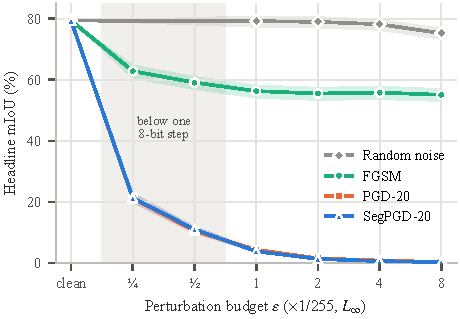
\includegraphics[width=\columnwidth]{figures/fig_miou_eps.pdf}
\caption{Headline mIoU as a function of the $L_\infty$ budget, with the 95\% bootstrap CIs shaded. The grey band marks the additional budgets below one 8-bit intensity step.}
\label{fig:eps}
\end{figure}

\subsection{Effect of the number of iterations}
The effect of the number of iterations is shown in Table~\ref{tab:ablation} and Fig.~\ref{fig:ablation}. The number of steps turns out to matter more than the budget: with five PGD steps at $\eps=1/255$ the mIoU already drops to \nPGDFiveOne\% ($-$\nPGDFiveOneFall\% relative), which is more than FGSM achieves with eight times the budget. The damage keeps increasing up to 40 steps (\nPGDFortyOne\% at $1/255$), so the results for 20 steps are conservative and should be read as an upper bound on the robustness of the model~\cite{croce2023reliable}. PGD and SegPGD give statistically indistinguishable mIoU values for every number of steps. SegPGD does, however, flip a larger share of the clean-correct pixels (\nCWSegMin--\nCWSegMax\% compared with \nCWPGDMin--\nCWPGDMax\% at $T=20$; Table~\ref{tab:main}), which is the behaviour its reweighted loss was designed for. For this model plain PGD is already strong enough to bring the mIoU close to zero, so the advantage of the segmentation-specific loss becomes visible in the pixel-flip rate rather than in the mIoU.

\begin{table}[t]
\centering
\caption{Headline mIoU (\%) for different numbers of attack iterations $T$. $^\ddagger$FGSM, i.e.\ one step of size $\eps$.}
\label{tab:ablation}
\footnotesize
\setlength{\tabcolsep}{4.5pt}
\begin{tabular}{@{}llrrrrr@{}}
\toprule
$\varepsilon$ & Attack & $T{=}1$ & 5 & 10 & 20 & 40 \\
\midrule
1/255 & PGD & 56.28$^\ddagger$ & 22.01 & 9.38 & 4.35 & 2.24 \\
1/255 & SegPGD & -- & 20.97 & 9.61 & 3.88 & 2.57 \\
\addlinespace[2pt]
4/255 & PGD & 55.81$^\ddagger$ & 9.71 & 2.73 & 0.84 & 0.34 \\
4/255 & SegPGD & -- & 8.99 & 2.48 & 0.68 & 0.33 \\
\bottomrule
\end{tabular}

\end{table}

\begin{figure}[t]
\centering
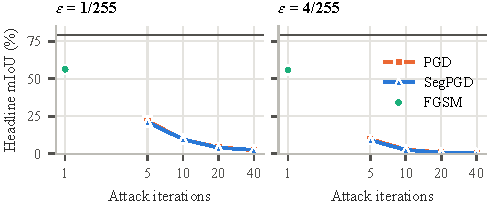
\includegraphics[width=\columnwidth]{figures/fig_ablation.pdf}
\caption{Step-count ablation at $\eps=1/255$ and $4/255$. The horizontal line shows the clean mIoU.}
\label{fig:ablation}
\end{figure}

\subsection{Anatomy versus instruments}
In Table~\ref{tab:groups} and Fig.~\ref{fig:groups} we compare the relative fall of the anatomy and instrument group means. As long as an attack is not saturated, the instruments lose a larger part of their clean accuracy than the anatomical structures. The difference is $+$\nGapNoiseEight\pp\ for noise at $8/255$, between $+$\nGapFGSMQ\ and $+$\nGapFGSMEight\pp\ for FGSM, and $+$\nGapPGDQ\pp\ (PGD-20) and $+$\nGapSegQ\pp\ (SegPGD-20) at $\eps=\frac14/255$. In the last case the anatomy mIoU falls by \nAnatFallPGDQ\% and the instrument mIoU by \nInstFallPGDQ\% under PGD-20. For all of these settings the bootstrap CI does not include zero, and the same direction is observed in all six test videos. The difference is also not caused by hallucinated instrument pixels. When each class is scored only on frames in which it is present, the gap at $\frac14/255$ becomes smaller but remains clearly positive, at $+$\nGapPresPGDQ\pp\ for PGD-20 and $+$\nGapPresSegQ\pp\ for SegPGD-20. Once the attacks saturate ($\eps\ge4/255$), both groups are close to zero and the difference disappears. It should also be noted that under strong attacks the anatomy loses more IoU in absolute terms, simply because its clean IoU is higher. Our question concerns how quickly each group degrades, and for this reason we use the relative fall as the main measure.

\begin{table}[t]
\centering
\caption{Relative fall (\%) of the anatomy and instrument group mIoU. $\Delta$ is the instrument value minus the anatomy value (pp) with a paired bootstrap 95\% CI; $\Delta_{\mathrm{pres}}$ is the same difference when each class is scored only on frames in which it is present; Vid.\ is the number of test videos (out of 6) in which the instruments fall further. $\eps$ in units of 1/255.}
\label{tab:groups}
\footnotesize
\setlength{\tabcolsep}{3.2pt}
\begin{tabular}{@{}lrrrrrr@{}}
\toprule
Attack & $\varepsilon$ & Anat. & Instr. & $\Delta$ [95\% CI] & $\Delta_{\mathrm{pres}}$ & Vid. \\
\midrule
Noise & 8 & 2.8 & 6.4 & $+3.6$ [$+2.2$, $+5.1$] & $+3.9$ & 6/6 \\
\addlinespace[1.5pt]
FGSM & $\frac{1}{4}$ & 15.3 & 23.6 & $+8.2$ [$+5.2$, $+11.2$] & $+7.1$ & 6/6 \\
FGSM & 1 & 21.2 & 33.0 & $+11.8$ [$+8.5$, $+15.1$] & $+10.2$ & 6/6 \\
FGSM & 8 & 19.5 & 36.1 & $+16.7$ [$+13.4$, $+20.0$] & $+15.3$ & 6/6 \\
\addlinespace[1.5pt]
PGD-20 & $\frac{1}{4}$ & 59.4 & 80.1 & $+20.7$ [$+16.8$, $+24.2$] & $+14.6$ & 6/6 \\
PGD-20 & 1 & 88.9 & 97.3 & $+8.4$ [$+6.4$, $+10.3$] & $+7.8$ & 6/6 \\
PGD-20 & 8 & 99.1 & 99.7 & $+0.7$ [$+0.2$, $+1.5$] & $+0.3$ & 4/6 \\
\addlinespace[1.5pt]
SegPGD-20 & $\frac{1}{4}$ & 62.3 & 78.4 & $+16.1$ [$+12.5$, $+19.6$] & $+12.5$ & 6/6 \\
SegPGD-20 & 1 & 91.2 & 97.0 & $+5.8$ [$+4.2$, $+7.4$] & $+6.0$ & 6/6 \\
SegPGD-20 & 8 & 99.2 & 99.8 & $+0.6$ [$+0.2$, $+1.2$] & $+0.4$ & 5/6 \\
\bottomrule
\end{tabular}

\end{table}

\begin{figure*}[t]
\centering
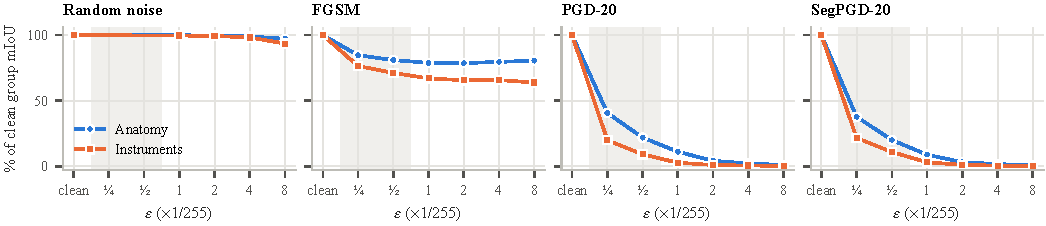
\includegraphics[width=\textwidth]{figures/fig_groups.pdf}
\caption{Fraction of the clean group mIoU that is retained under each attack (anatomy: blue circles; instruments: orange squares). The grey band marks the sub-8-bit budgets.}
\label{fig:groups}
\end{figure*}

\begin{figure*}[t]
\centering
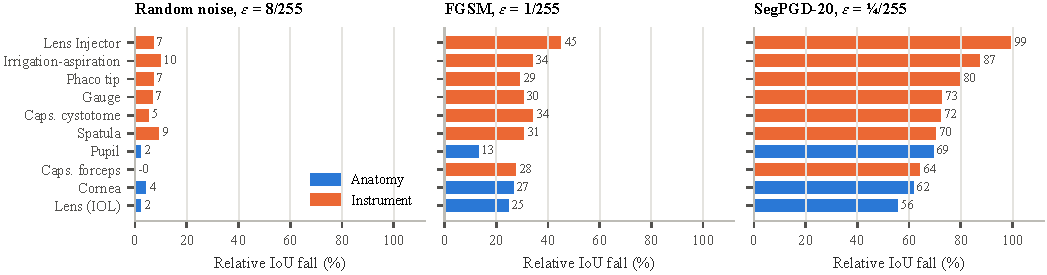
\includegraphics[width=\textwidth]{figures/fig_class_fall.pdf}
\caption{Relative IoU fall per class in three regimes in which the attacks are not saturated (headline classes only). The anatomical classes (blue) are among the least affected in all three cases; among the instruments, the capsulorhexis forceps is an exception.}
\label{fig:classes}
\end{figure*}

Fig.~\ref{fig:classes} shows the same comparison for the individual classes. In each of the three regimes the anatomical classes are among the least affected. Under FGSM at $1/255$ the anatomy group falls by \nAnatFallFGSMOne\% and the instrument group by \nInstFallFGSMOne\%; the lens injector is the most fragile class ($-45\%$), followed by the capsulorhexis cystotome and the irrigation--aspiration handpiece ($-34\%$ each). The capsulorhexis forceps, although it is thin and metallic, behaves more like the anatomy. Across classes, the mean object area and the relative fall are negatively correlated in every unsaturated run (Spearman $\rho$ between \nRhoMin\ and \nRhoMax), so smaller structures tend to fall further. With only ten classes, however, none of these correlations is significant (the smallest $p$-value is \nRhoPMin). We therefore regard the higher vulnerability of the instruments as a reliable group-level effect, while object size is a plausible explanation that our data cannot confirm. The absolute per-class IoU values behind Fig.~\ref{fig:classes} are given in Table~\ref{tab:perclass}.

\begin{table}[t]
\centering
\caption{Per-class IoU (\%) on the held-out test fold without attack and under attack ($\eps$ in units of 1/255; PGD and SegPGD with $T=20$). $^\ast$Rare class.}
\label{tab:perclass}
\footnotesize
\setlength{\tabcolsep}{2.2pt}
\begin{tabular}{@{}lrrrrrr@{}}
\toprule
Class & Clean & Noise 8 & FGSM 1 & PGD $\frac{1}{4}$ & SegPGD $\frac{1}{4}$ & SegPGD 1 \\
\midrule
Cornea & 84.5 & 81.1 & 62.1 & 36.2 & 32.4 & 7.4 \\
Pupil & 92.4 & 90.4 & 80.4 & 31.2 & 28.4 & 4.7 \\
Lens (IOL) & 86.6 & 84.7 & 65.2 & 39.7 & 38.5 & 11.0 \\
\addlinespace[2pt]
Slit/inc. knife$^\ast$ & 79.2 & 80.5 & 61.8 & 13.6 & 15.0 & 6.4 \\
Gauge & 70.4 & 65.7 & 49.0 & 19.1 & 19.3 & 1.5 \\
Caps. cystotome & 64.6 & 61.3 & 42.6 & 19.7 & 17.9 & 1.2 \\
Caps. forceps & 75.0 & 75.3 & 54.2 & 23.2 & 26.9 & 1.0 \\
Katena Forceps$^\ast$ & 4.1 & 4.0 & 4.0 & 4.1 & 4.2 & 3.3 \\
Spatula & 74.4 & 67.5 & 51.5 & 17.5 & 22.1 & 5.4 \\
Phaco tip & 82.9 & 77.2 & 58.8 & 14.4 & 16.9 & 4.8 \\
Irrigation-asp. & 84.1 & 75.8 & 55.7 & 10.7 & 10.7 & 1.7 \\
Lens Injector & 78.6 & 73.1 & 43.2 & 0.8 & 0.5 & 0.2 \\
\bottomrule
\end{tabular}

\end{table}

\subsection{Failure modes: hallucination and mislocalisation}
Table~\ref{tab:composition} lists the fraction of pixels assigned to each class. FGSM hardly changes these fractions, even though it removes about 30\% of the mIoU, which means that it mainly shifts and confuses the predicted structures. The iterative attacks behave differently and make the model hallucinate. Under SegPGD-20 at $4/255$, \nPupilSeg\% of all pixels are labelled as pupil although the true fraction is \nPupilGT\%, \nInjSeg\% are labelled as lens injector (true fraction \nInjGT\%), and the background fraction drops from \nBgGT\% to \nBgSeg\%. Examples are shown in Fig.~\ref{fig:qual}. The adversarial frames cannot be told apart from the clean frames, but the predicted scenes have little in common with the actual surgery. For downstream applications such as tool tracking or phase recognition, false structures predicted with high confidence are arguably more harmful than an empty mask.

\begin{table}[t]
\centering
\caption{Fraction of test pixels (\%) assigned to each class at $\eps=4/255$. Values more than three times the ground-truth fraction are printed in bold.}
\label{tab:composition}
\footnotesize
\setlength{\tabcolsep}{4pt}
\begin{tabular}{@{}lrrrrr@{}}
\toprule
Class & GT & Clean & FGSM & PGD-20 & SegPGD-20 \\
\midrule
Background & 84.8 & 84.9 & 85.1 & 40.3 & 33.6 \\
Cornea & 5.5 & 5.5 & 5.5 & 5.6 & 6.3 \\
Pupil & 6.7 & 6.6 & 6.8 & \textbf{43.7} & \textbf{49.5} \\
Lens (IOL) & 0.9 & 0.9 & 0.8 & 0.4 & 0.4 \\
Gauge & 0.1 & 0.1 & 0.1 & \textbf{1.1} & \textbf{0.6} \\
Spatula & 0.4 & 0.4 & 0.3 & 0.9 & 1.1 \\
Phaco tip & 0.6 & 0.6 & 0.5 & 0.7 & 1.1 \\
Lens Injector & 0.1 & 0.1 & 0.1 & \textbf{5.4} & \textbf{6.0} \\
\bottomrule
\end{tabular}

\end{table}

\begin{figure*}[t]
\centering
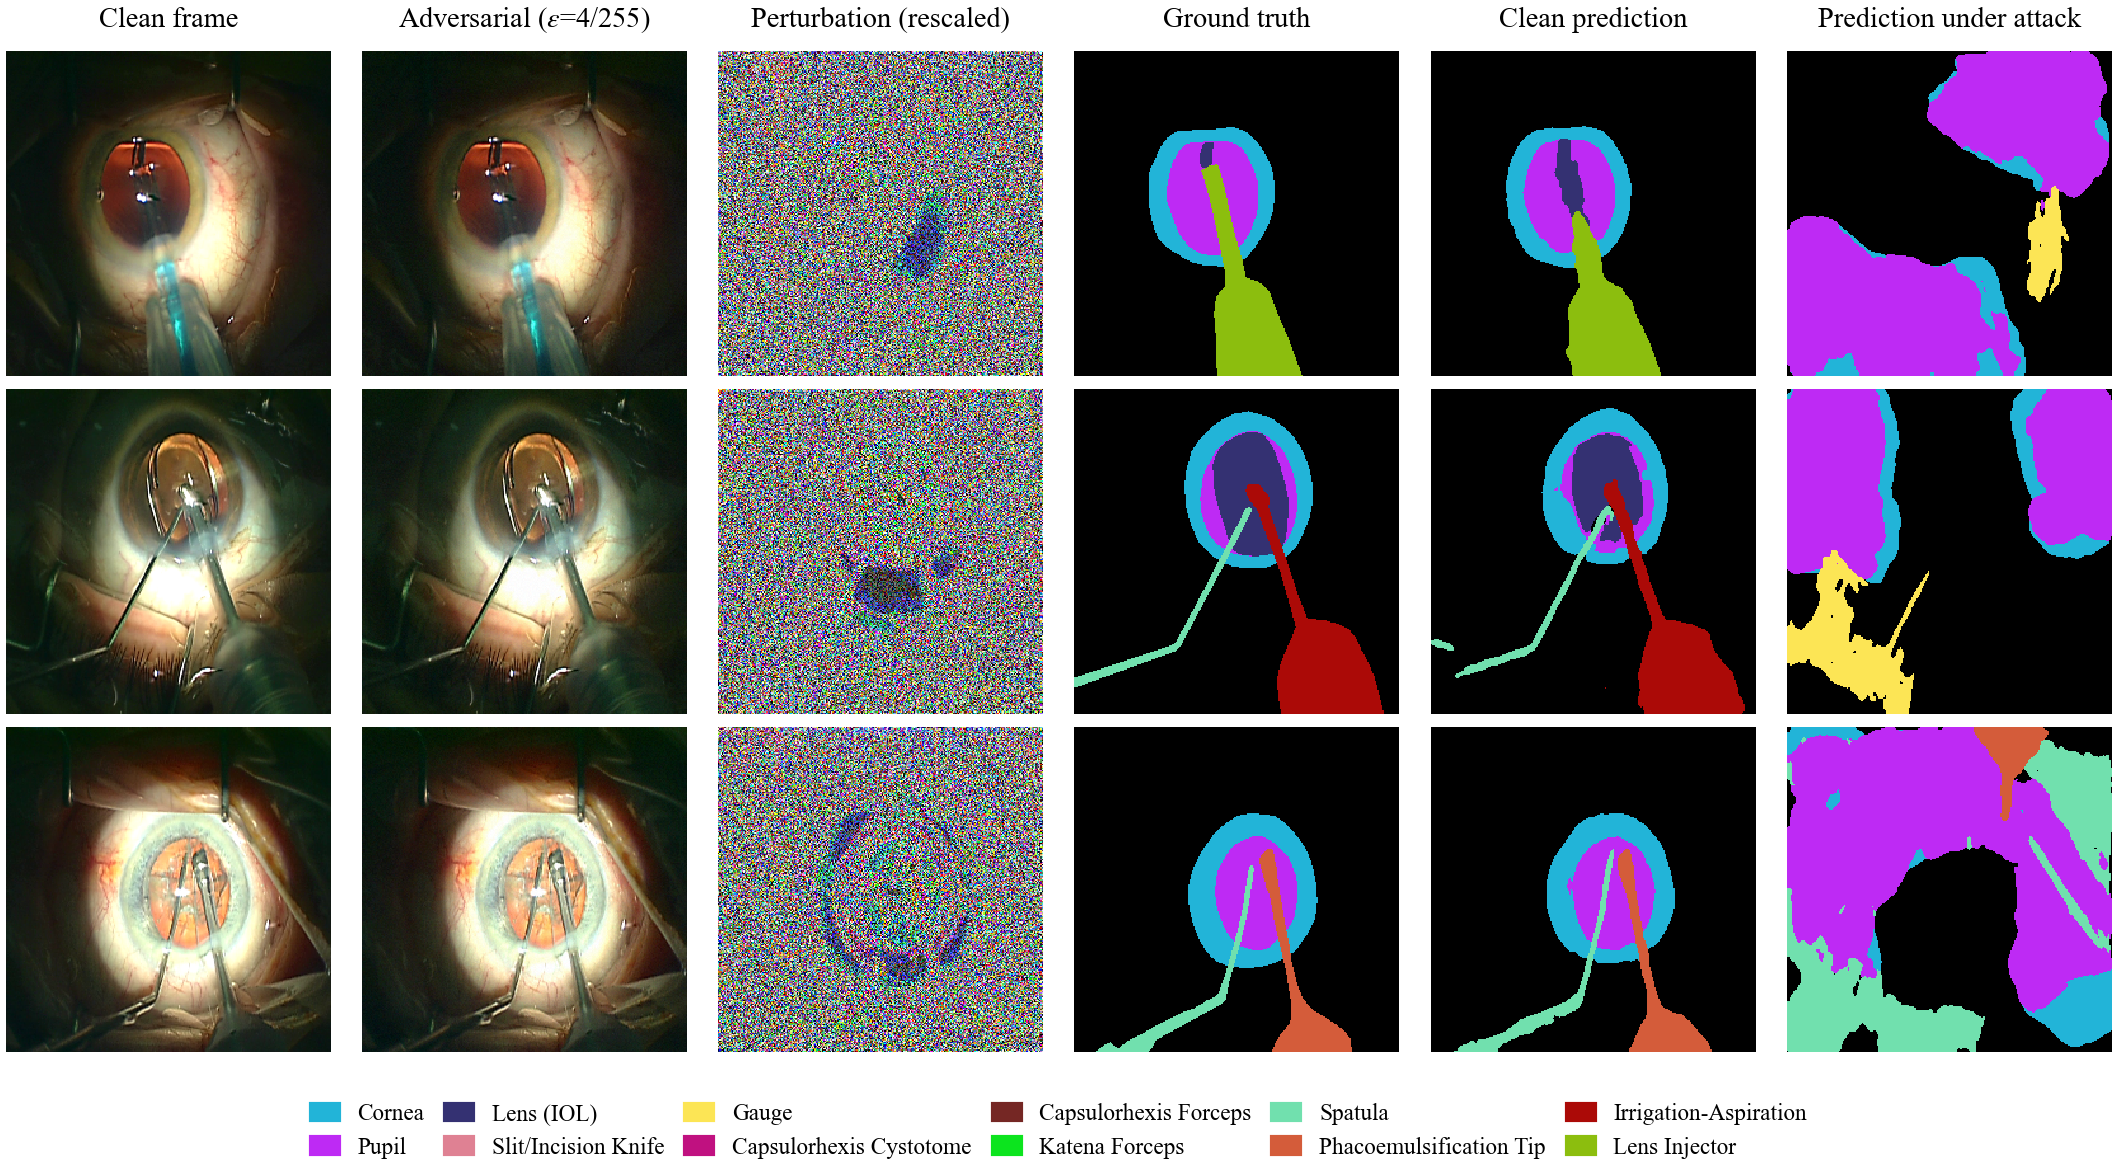
\includegraphics[width=\textwidth]{figures/fig_qualitative.png}
\caption{SegPGD-20 at $\eps=4/255$ on three test frames. For visibility, the perturbation is rescaled from $\pm\eps$ to the full intensity range. Although the adversarial frames look the same as the clean frames, the predictions consist largely of hallucinated regions. In row~3 the Katena forceps (green, top left of the ground truth) is missed already by the clean model.}
\label{fig:qual}
\end{figure*}

\subsection{Additional checks}
In Table~\ref{tab:checks}(a) the adversarial frames are rounded to 8-bit values before inference, as would happen if they were stored as images. The mIoU changes by at most \nQuantMax\pp, so the results do not depend on floating-point precision. Table~\ref{tab:checks}(b) compares the full-data results with an earlier run of the same pipeline on an independent subset of 908 frames (524 for training and 259 for testing). All of the main vulnerability results are reproduced. In both runs the iterative attacks remove about 95\% of the mIoU at $1/255$, FGSM removes about one third, and the model hallucinates under attack. Two secondary results changed. The anatomy--instrument gap under iterative attacks was inconclusive on 908 frames (four of six videos) but is clear on the full data (six of six). In addition, the smaller model was roughly twice as sensitive to random noise (\nRepNoiseEight\% vs.\ \nNoiseEightFall\% at $8/255$), while its vulnerability to PGD was the same (\nRepPGDOne\% vs.\ \nPGDOneFall\%).

\begin{table}[t]
\centering
\caption{Additional checks: (a) 8-bit quantisation of the adversarial frame; (b) repetition of the study on an independent run with 908 frames.}
\label{tab:checks}
\footnotesize
\setlength{\tabcolsep}{3.5pt}
\begin{tabular}{@{}lrr@{}}
\toprule
\multicolumn{3}{@{}l}{\emph{(a) 8-bit quantisation of the adversarial frame}} \\
mIoU (\%) & Float & 8-bit \\
\midrule
PGD-20, $\varepsilon$ = 1/255 & 4.35 & 4.09 \\
PGD-20, $\varepsilon$ = 2/255 & 1.57 & 1.65 \\
SegPGD-20, $\varepsilon$ = 1/255 & 3.88 & 3.75 \\
SegPGD-20, $\varepsilon$ = 2/255 & 1.38 & 1.53 \\
FGSM, $\varepsilon$ = 1/255 & 56.28 & 56.28 \\
FGSM, $\varepsilon$ = 2/255 & 55.49 & 55.48 \\
\midrule
\multicolumn{3}{@{}l}{\emph{(b) Replication on an independent run}} \\
Quantity & 908 frames & Full data \\
\midrule
Clean mIoU (\%) & 77.08 & 79.35 \\
Noise 8/255: rel.\ fall (\%) & 10.3 & 5.2 \\
FGSM 1/255: rel.\ fall (\%) & 34.0 & 29.1 \\
PGD-20 1/255: rel.\ fall (\%) & 95.0 & 94.5 \\
SegPGD-20 1/255: rel.\ fall (\%) & 95.1 & 95.1 \\
FGSM 1/255: gap, pp (videos) & $+9.7$ (6/6) & $+11.8$ (6/6) \\
PGD-20 $\frac{1}{4}$/255: gap, pp (videos) & $+8.7$ (4/6) & $+20.7$ (6/6) \\
SegPGD-20 4/255: pupil share (\%) & 41.2 & 49.5 \\
\bottomrule
\end{tabular}

\end{table}

% ==============================================================================================
\section{Discussion}

\subsection{Clean accuracy and reliability}
A model that matches or exceeds the published benchmark on clean frames loses 95\% of its segmentation quality under a perturbation of a single intensity level, and still 73\% under a quarter of one level. Perturbations of this size are far below what a human observer can perceive, so inspecting the frames would not reveal them. This agrees with earlier reports on the vulnerability of medical models~\cite{finlayson2018adversarial,ma2021understanding} and suggests that the problem carries over from diagnostic images to intra-operative video.

\subsection{Why the instruments are more fragile}
Instruments are thin and specular and cover only a small number of pixels, so flipping a few pixels already removes a large part of their area. The anatomical structures, in comparison, are large, nested (the pupil lies inside the cornea) and strongly constrained by their context. The negative correlation between object size and vulnerability that we observed consistently is in line with this explanation. The capsulorhexis forceps, however, is thin and still robust, which suggests that size alone does not determine vulnerability and that appearance and contextual cues also play a role.

\subsection{Hallucinated predictions}
Under the iterative attacks the model replaces the scene with large and confident structures that are anatomically implausible. For downstream analysis this is more problematic than a missing prediction. At the same time it may offer a way to detect attacks, because the hallucinated layouts violate basic anatomical constraints. This would be consistent with the observation of Ma \emph{et al.}~\cite{ma2021understanding} that adversarial examples for medical images can be easier to detect.

\subsection{Training data and robustness}
The full-data model, which was trained on 2.7 times more frames, was about half as sensitive to random noise as the 908-frame model, but equally vulnerable to the iterative attacks. The two runs also differ in the training schedule and in the size of the test set. Still, the comparison suggests that more clean data alone will not provide robustness against worst-case perturbations, and that explicit defences such as adversarial training, for which SegPGD was also proposed~\cite{gu2022segpgd}, will be required.

\subsection{Threat scenarios}
The white-box setting represents a worst case, but two of our results bring it closer to practice. First, the perturbations survive rounding to 8-bit pixel values, so they could be contained in stored or streamed frames and do not have to be injected directly into the input of the model. Second, only a few gradient steps are needed (five PGD steps at $1/255$ already remove \nPGDFiveOneFall\% of the mIoU). Every component that can modify the video between the microscope camera and the segmentation model, for example recording software, a network relay or an analysis server, would therefore have to be regarded as part of the attack surface. Whether such perturbations transfer to other models, and whether they survive lossy video compression, are open questions that could be studied with the protocol used here.

\subsection{Implications for evaluation}
Since single-step attacks reach only about one third of the damage and 20-step attacks still improve at 40 steps, claims about the robustness of surgical segmentation models should be based on strong iterative attacks, and the number of steps should be reported, as has been argued for natural images~\cite{croce2023reliable,athalye2018obfuscated}. Reporting the pixel-flip rate in addition to the mIoU is also helpful, because it reveals differences between attacks that the mIoU no longer reflects once it is saturated. We would suggest that benchmarks for surgical segmentation such as Cataract-1K report, in addition to the clean accuracy, at least the mIoU under random noise and under PGD at $\eps=1/255$. Both are cheap to compute and, as our results show, can lead to very different conclusions than the clean accuracy alone. Since transformer-based segmentation models were found to be more robust than convolutional ones on volumetric data~\cite{malik2024evaluating}, a comparison of architectures under the same protocol would be a useful next step.

% ==============================================================================================
\section{Limitations}
Our study has several limitations. We evaluated a single architecture, a single training seed and only the official test fold, so the variance across folds is not known; the independent run on 908 frames compensates for this only in part. Frames from the same video are correlated, which is why we consider the per-video counts the more conservative evidence. Two instrument classes are too rare in the test fold to draw conclusions for them individually. The threat model is a digital white-box worst case in which the attacker also has access to the ground-truth labels. Black-box, transfer, physical and temporal attacks were not evaluated, and perturbations below one 8-bit step are only possible if the decoded frames themselves are manipulated. The comparison with the published benchmark is not like-for-like. Finally, all measurements were made on recorded video in a laboratory setting and do not by themselves allow conclusions about patient safety.

% ==============================================================================================
\section{Conclusion}
We have studied the adversarial robustness of cataract surgical scene segmentation on the Cataract-1K benchmark. A DeepLabV3+ baseline with good clean accuracy drops from \nCleanMIoU\% to about 4\% mIoU when each pixel is perturbed by one intensity level, the attack still works after the frames are stored with 8-bit precision, and the attacked model produces hallucinated structures instead of failing silently. Surgical instruments were consistently more vulnerable than the surrounding anatomy, and a larger amount of clean training data did not improve the adversarial robustness. In future work we plan to evaluate defences such as adversarial training and the detection of implausible predictions, black-box and transfer attacks, attacks that exploit the temporal structure of video, and further architectures, including foundation models attacked with region-aware methods.

\section*{Acknowledgment}
We thank the authors of the Cataract-1K dataset and Klinikum Klagenfurt for making the data publicly available.

% Balance the two columns on the last page (IEEE practice): start a new column at reference 18.
\IEEEtriggeratref{18}
\bibliographystyle{IEEEtran}
\bibliography{refs}

\end{document}
